\documentclass[12pt,oneside,slovak,a4paper]{article}

\usepackage[slovak]{babel}
\usepackage[utf8]{inputenc}
\usepackage{amsmath}
\usepackage{amsfonts}
\usepackage{amssymb}
\usepackage{graphicx}
\usepackage{cite}
\usepackage[IL2]{fontenc} % lepšia sadzba písmena Ľ než v T1
\usepackage{pdfpages}
\usepackage{url} % príkaz \url na formátovanie URL
\usepackage[hidelinks]{hyperref} % odkazy v texte budú aktívne (pri niektorých triedach dokumentov spôsobuje posun textu)
\usepackage[left=2cm,right=2cm,top=2cm,bottom=2cm]{geometry}
\usepackage{float}
\usepackage[normalem]{ulem}
\useunder{\uline}{\ul}{}
\usepackage{titling}
\usepackage{xcolor}
\usepackage{lipsum}
\usepackage{setspace}
\usepackage{blindtext}
\usepackage{caption}
\usepackage{tabularx}
\usepackage[numbers]{natbib}

% riadkovanie 1.5
\begin{document}
\linespread{1.5}\selectfont

\begin{titlepage}
	\centering
    {\Large Slovenská technická univerzita v Bratislave\par}
    {\Large Fakulta informatiky a informačných technológií\par}
	\vspace{7cm}
	{\huge\bfseries Voľne šíriteľné nástroje na obnovu zmazaných súborov\par}
	\vspace{0.5cm}
    {\Large \textsc{Princípy informačnej bezpečnosti}\par}
    \vspace{1cm}
	{\Large\itshape Marek Čederle\par}
    {\small\texttt{xcederlem@stuba.sk}\par}
	\vfill

	{\large \today\par}
\end{titlepage}


\tableofcontents
\vspace*{\fill}

% ----------------- 1. kapitola -----------------

% vsetky zdroje z literatura.bib aby sa zobrazili bez citovania
\nocite{*}

\section{Špecifikácia projektu}
V mojom projekte sa budem venovať analýze súborových systémov pre operačné systémy Windows a GNU+Linux. Bude sa jednať o súborové systémy typu NTFS a ext ale spomeniem aj dodnes veľmi používané FAT32 a exFAT ktoré sa používajú na prenosných médiách. Každý súborový systém by som chcel opísať s tým, že uvediem jeho výhody a nevýhody prípadné porovnanie s ďalšími spomenutými súborovými systémami.

Budem sa zaoberať aj tým, ako správne naformátovať disk (prepísať ho náhodnými dátami alebo samými nulami) aby pri jeho predaji sa z bezpečnostných dôvodov nedalo zistiť čo sa na ňom pred tým nachádzalo. Je to z dôvodu že pri mazaní dát z disku sa vlastne tieto dáta reálne nemažú. Dáta na disku zostanú, len sa z tabuľky záznamov zahodí záznam kde sa súbor nachádza a potom keď sa zapisuje na disk tak operačný systém vie, že môže na toto miesto zapisovať. 

Taktiež sa budem zaoberať analýzou nástroja na obnovu zmazaných súborov s názvom testdisk. Vysvetlím, prečo som si vybral práve tento nástroj. S týmto nástrojom budem následne experimentovať. Experimenty budú spočívať v tom, že si naformátujem disk a vytvorím na ňom nejaké partície podľa typu daného súborového systému. Následne naň uložím rôzne typy súborov. Budú sa tam nachádzať fotky, textové súbory, archívy, atď. Potom vymažem nejaké z týchto súborov, ale na disk ďalej nič nezapíšem, aby sa nezačali prepisovať dané miesta na disku inými súbormi. Následne vyskúšam nástroj na obnovu zmazaných súborov (testdisk) či zvládne tieto súbory obnoviť. Tento experiment zopakujem s tým, že po zmazaní ďalších súborov zapíšem na disk zase nové súbory a vyskúšam použiť nástroj na obnovu či dokáže aj po takejto akcii obnoviť súbory. Ďalší experiment bude spočívať v zmazaní celej partície a jej následnej obnove týmto nástrojom. V neposlednom rade ukážem, že po správnom formátovaní disku sa nebudú dať dáta obnoviť. Na záver budem prezentovať výsledky experimentov.
\subsection{Progress report č.1}
V prvom progress reporte vypracujem teoretickú časť, ktorú som na začiatku uviedol. To znamená popísanie rôznych typov súborových systémov a nástrojov na obnovu súborov. V neposlednom rade uvediem ako z bezpečnostného hľadiska správne ``zmazať'' súbory na disku respektíve ako ho naformátovať tak, aby sa z neho minulé dáta nedali prečítať.

\subsection{Progress report č.2}
V tomto progress reporte sa budem zameriavať na praktickú/experimentálnu časť. To znamená, že sa pokúsim vykonať všetky vyššie spomenuté experimenty. Na záver budem pracovať na celkovej úprave finálneho dokumentu.

\subsection{Ciele projektu}
Cieľom tohto projektu je získať informácie z oblasti súborových systémov a vykonať rôzne experimenty s nástrojmi na obnovu údajov. Keďže sa jedná o predmet Princípy informačnej bezpečnosti, tak cieľom je poukázať na dopady neformátovania respektíve neefektívneho ``ničenia'' súborov na bezpečnosť.

% ----------------- 2. kapitola -----------------

\section{Súborové systémy}
Súborový systém je metóda a dátová štruktúra, ktorú operačný systém používa na riadenie spôsobu ukladania a načítavania dát. Bez súborového systému by dáta umiestnené na pamäťovom médiu boli jedným veľkým zväzkom dát bez možnosti určiť, kde končí jeden súbor a začína ďalší, alebo kde sa nachádza, keď je potrebné ho načítať. Rozdelením dát na časti a pomenovaním každej časti sa dáta ľahko izolujú a identifikujú. Každá skupina dát sa nazýva súbor.

\subsection{FAT - File Allocation Table}
FAT je súborový systém vyvinutý pre osobné počítače. Pôvodne vyvinutý v roku 1977 na použitie na disketách, neskôr bol prispôsobený na použitie na pevných diskoch a iných zariadeniach. Často je z dôvodov kompatibility podporovaný súčasnými operačnými systémami pre osobné počítače a mnohými mobilnými zariadeniami a ``embed'' systémami. FAT ako taký je už v dnešnej dobe nepoužívaný, ale jeho odnože (FAT32, exFAT) sa doteraz používajú napríklad v prenosných médiách ako USB kľúče, SD karty a podobne.

\subsubsection{FAT32}
Najpokročilejšia verzia súborového systému FAT je FAT32. S FAT32 sa Microsoft snažil prekonať obmedzenia FAT16 a prispôsobiť sa väčším možným partíciám. Existuje už od Windowsu 95 a naďalej zostáva populárny, pretože je vysoko kompatibilný s väčšinou operačných systémov (GNU+Linux, MAC) a prenosných zariadení. FAT32 podporuje súbory menšie ako 4 GB a partície s maximálnou veľkosťou 2 TB.

\subsubsection{Štruktúra FAT a FAT32}
Novo naformátovaný disk s FAT vyzerá nasledovne:

\begin{figure}[H]
	\centering
	\captionsetup{justification=centering,margin=2cm}
	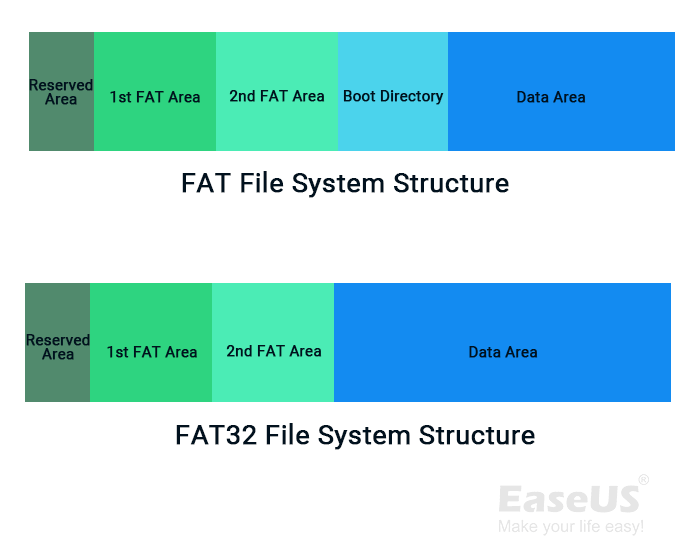
\includegraphics[width=\linewidth]{./images/fat-file-system-structure.png}
	\centering
	\caption{Štruktúra súborového systému FAT a FAT32 \\ Zdroj: https://www.easeus.com/diskmanager/file-system.html}
\end{figure}

\setstretch{1.0}
\begin{itemize}
	\item Reserved Area
		\begin{itemize}
			\item Obsahuje boot sector, BPB (BIOS Parameter Block) a celkovo informácie potrebné pre bootovanie a súborový systém.
		\end{itemize}
	\item 1st FAT Area
		\begin{itemize}
			\item FAT tabuľka obsahujúca informácie o súboroch a ich umiestnení na disku.
		\end{itemize}
	\item 2nd FAT Area
		\begin{itemize}
			\item Obsahuje kópiu FAT tabuľky.
		\end{itemize}
	\item Boot Directory
		\begin{itemize}
			\item Niekedy sa nazýva aj Root Directory. Používa sa iba v derivátoch FAT12 a FAT16. Obsahuje informácie o súboroch, ktoré sa nachádzajú priamo v koreňovom adresári.
		\end{itemize}
	\item Data Area
		\begin{itemize}
			\item Obsahuje samotné dáta súborov.
		\end{itemize}
\end{itemize}

\subsubsection{exFAT - Extensible File Allocation Table}
exFAT je súborový systém predstavený spoločnosťou Microsoft v roku 2006 a optimalizovaný pre flash pamäte, ako sú USB flash disky a SD karty. exFAT bol proprietárny do 28. augusta 2019, kedy Microsoft zverejnil jeho špecifikáciu. Microsoft však stále vlastní patenty na niekoľko častí svojho dizajnu.

exFAT možno použiť tam, kde NTFS nie je vhodným riešením (kvôli vysokej réžii\footnote{angl. overhead}), ale kde je potrebná podpora súborov väčších ako 4 GB.

exFAT bol prijatý SD Association ako predvolený súborový systém pre karty SDXC väčšie ako 32 GB.

Windows 8 a novšie verzie natívne podporujú bootovanie z exFAT.

\subsubsection{Štruktúra exFAT}
Novo naformátovaný disk s exFAT vyzerá nasledovne:

\begin{figure}[H]
	\centering
	\captionsetup{justification=centering,margin=2cm}
	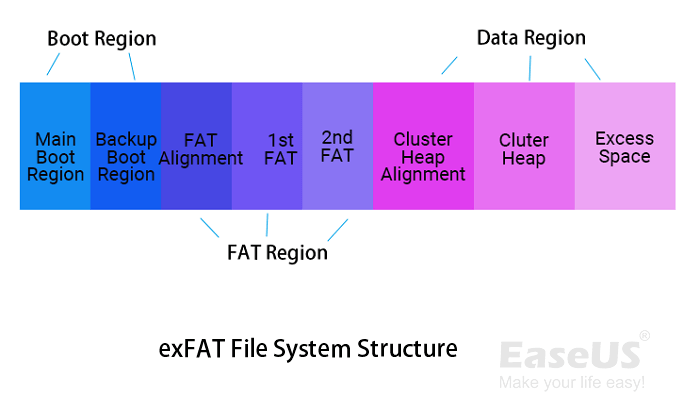
\includegraphics[width=\linewidth]{./images/exfat-file-system-structure.png}
	\centering
	\caption{Štruktúra súborového systému exFAT \\ Zdroj: https://www.easeus.com/diskmanager/file-system.html}
\end{figure}

\setstretch{1.0}
\begin{itemize}
	\item Main Boot Region
		\begin{itemize}
			\item Informácie potrebné pre bootovanie.
		\end{itemize}
	\item Backup Boot Region
		\begin{itemize}
			\item Záloha Main Boot Region.
		\end{itemize}
	\item FAT Alignment
		\begin{itemize}
			\item FAT offset a veľkosť.
		\end{itemize}
	\item 1st FAT
		\begin{itemize}
			\item FAT tabuľka obsahujúca informácie o súboroch a ich umiestnení na disku.
		\end{itemize}
	\item 2nd FAT
		\begin{itemize}
			\item Záloha FAT tabuľky.
		\end{itemize}
	\item Cluster Heap Alignment
		\begin{itemize}
			\item Cluster heap offset a veľkosť.
		\end{itemize}
	\item Cluster Heap
		\begin{itemize}
			\item Obsahuje samotné dáta súborov.
		\end{itemize}
\end{itemize}

\subsubsection{Výhody a nevýhody FAT32 a exFAT}
% dorobit
% tabulka pre FAT32

% tabulka pre exFAT


\subsection{NTFS - New Technology File System}
NTFS je proprietárny súborový systém vytvorený spoločnosťou Microsoft. Bol uvedený s vtedy novým operačným systémom Windows NT\footnote{New Technology} v roku 1993. Vtedy nahradil dovtedy veľmi používaný súborový systém FAT. NTFS je predovšetkým určený pre pevné disky HDD\footnote{Hard Disk Drive} a neskôr aj pre SSD\footnote{Solid State Drive}. Je však možné ho použiť aj na prenosové média typu USB kľúč a podobne. 


Súborový systém NTFS prináša kombináciu vyššej rýchlosti, väčšej spoľahlivosti a kompatibility oproti súborovému systému FAT, ktorý bol jeho predchodcom v ére operačného systému MS DOS.

\subsubsection{Štruktúra NTFS}
Novo naformátovaný disk s NTFS vyzerá nasledovne:

\begin{figure}[H]
	\centering
	\captionsetup{justification=centering,margin=2cm}
	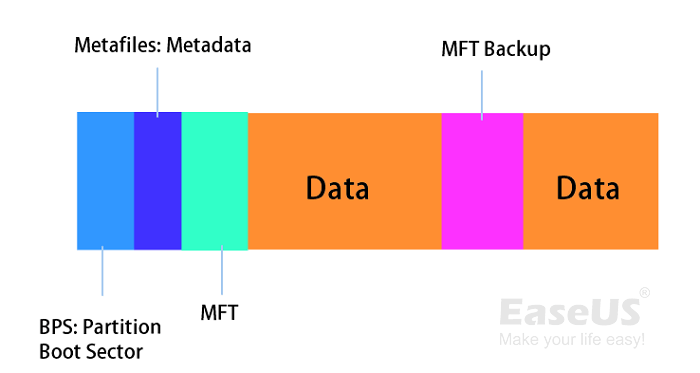
\includegraphics[width=\linewidth]{./images/ntfs-file-system-structure.png}
	\centering
	\caption{Štruktúra súborového systému NTFS \\ Zdroj: https://www.easeus.com/diskmanager/file-system.html}
\end{figure}

% bulleted list plus riadkovanie iba na danu cas textu
\setstretch{1.0}
\begin{itemize}
	\item Partition Boot Sector
		\begin{itemize}
			\item Obsahuje informácie potrebné pre bootovanie. Primárne sa jedná o BootStrap čo je vlastne malý program, ktorý ma za úlohu načítať operačný systém do pamäte.
		\end{itemize}
	\item Metadata
		\begin{itemize}
			\item Pomáhajú definovať a organizovať súborový systém, zálohovať kritické údaje súborového systému.
		\end{itemize}
	\item Master File Table (MFT)
		\begin{itemize}
			\item Obsahuje záznamy o všetkých súboroch a adresároch na disku. Je to v podstate ekvivalent FAT tabuľky.
		\end{itemize}
	\item Data
		\begin{itemize}
			\item Obsahuje samotné dáta súborov.
		\end{itemize}
	\item MFT Backup
		\begin{itemize}
			\item Obsahuje zálohu MFT tabuľky.
		\end{itemize}
\end{itemize}

\subsubsection{Bezpečnosť NTFS}
Súborový systém NTFS umožňuje nastaviť povolenia na prístup k niektorým lokálnym súborom a priečinkom. Inými slovami, dôverný súbor môžete nastaviť tak, aby bol pre niektorých iných používateľov nedostupný.

% Mozno este toto pridat
% Pouziva ACL encryption a podobne
% pridat sem o EFS (Encrypting File System) z https://www.ntfs.com/ntfs-encrypted.htm
% obnova dát https://www.ntfs.com/data-integrity.htm


\subsubsection{Výhody a nevýhody NTFS}

% tabulka s výhodami a nevýhodami
\begin{table}[H]
\begin{tabularx}{\linewidth}{|X|X|}
\hline
\multicolumn{1}{|c|}{\textbf{Výhody}} & \multicolumn{1}{c|}{\textbf{Nevýhody}} \\ \hline
Podporuje veľmi veľké súbory a nemá takmer žiadne reálne obmedzenie veľkosti oddielu. & Má uzatvorený zdrojový kód. \\ \hline
Poskytuje vylepšené zabezpečenie údajov pomocou funkcií riadenia úrovne prístupu a natívneho šifrovania. & Mac OS dokáže čítať jednotky naformátované v systéme NTFS, ale na systém NTFS je možné zapisovať iba prostredníctvom softvéru tretej strany. \\ \hline
Podporuje automatickú kompresiu súborov, čo umožňuje rýchlejší prenos súborov a väčší úložný priestor na disku. & Prenosné zariadenia, ako sú smartfóny so systémom Android a digitálne fotoaparáty, ho nepodporujú. \\ \hline
Umožňuje diskové kvóty, ktoré firmám poskytujú väčšiu kontrolu nad úložným priestorom. & Kompatibilita so systémami založenými na GNU+Linux síce existuje ale iba kvôli vôli softvérových inžinerov urobiť ovladače vďaka reverznému inžinierstvu. \\ \hline
Umožňuje používateľom sledovať pridané, upravené alebo odstránené súbory na disku. &  \\ \hline
Zameriava na konzistenciu súborového systému, takže v prípade výpadku napájania alebo zlyhania systému môžete rýchlo obnoviť svoje údaje. &  \\ \hline
\end{tabularx}
\centering
\captionsetup{justification=centering,margin=2cm}
\caption{Výhody a nevýhody súborového systému NTFS \\ Zdroj: https://superops.com/ntfs-vs-fat32}
\end{table}
% ------------- koniec tabulky -------------

\subsection{ext - Extended File System}


% ----------------- 3. kapitola -----------------

\section{Nástroje na obnovu údajov}


\subsection{Testdisk}


\subsection{(Pripadne Nejaký iný nástroj..)}


\section{Analýza nástroja na obnovu údajov - testdisk (táto sekcia tu asi nebude, keďže to už mám vyššie)}

\section{Experimentovanie s nástrojom testdisk}


\subsection{Zmazanie a obnova súborov}


\subsection{Zmazanie a obnova partície}


\section{Výsledky experimentov}
sem napisat vysledky a nakoniec napisat toto: ak spravne naformatujeme disk tak ze ho pomocou nejakeho nastroja prepiseme cey viacej krat nahodnymi datami tak je mozne ho predat bez obavy ze sa z neho daju obnovit data ktore tam boli pred tym, je to preto lebo pri vymazavani sa v "mazu" v podstate iba zaznami o danych suboroch repsketive sa oznacia ze tam je teraz volne miesto a moze sa tam zapisovat

\section{Záver}
ak sa nam stalo ze sme omylom vymazali particiu alebo subory ktore sme nechceli tak treba hned prestat zapisovat na disk a je velka sanca ze data vieme zachranit avsak ak zacneme robit zmeny na disku a nasledne nan zapisovat tak je v podstate jedno aky suborovy system pouzivame v kazdom pripade prepiseme data ktore tam boli


\bibliography{literatura}
\bibliographystyle{unsrtnat}
\end{document}